\section{Actuators}

Effectors are responsible for altering the state of the environment, with actuators facilitating the actions of effectors.
In robotics, we employ various types of actuators:
\begin{itemize}
    \item \textit{Electric motors}: these devices convert electrical energy into mechanical energy by leveraging the principles of electromagnetism. 
        They produce rotational motion through the interaction between magnetic fields and electric currents.
    \item \textit{Hydraulics}: this technology utilizes fluids to transmit force, employing the principles of fluid mechanics to generate, control, and transfer power via pressurized liquids.
    \item \textit{Pneumatics}: a branch of engineering that employs compressed air or gas to transmit and regulate power, akin to hydraulics but using air or gas instead of liquids.
    \item \textit{Photo-reactive materials}: these substances undergo a chemical change upon exposure to light.
    \item \textit{Chemically reactive materials}: substances in this category undergo chemical reactions with other materials or their surroundings.
    \item \textit{Thermally reactive materials}: these substances undergo changes in properties or behavior when subjected to variations in temperature.
    \item \textit{Piezoelectric materials}: materials that generate electric charges in response to mechanical stress or pressure, while also displaying mechanical deformation under an electric field.
\end{itemize}

Originally, early robots were equipped with hydraulic and pneumatic actuators. 
Hydraulic actuators were costly, heavy, and required significant maintenance, making them suitable mainly for larger robots. 
Pneumatic actuators found use in stop-to-stop applications like pick-and-place tasks due to their swift actuation.

In modern times, electrical motors have become the prevalent choice for actuators. 
Typically, each joint incorporates its dedicated motor along with a controller. 
High-speed motors are often paired with elastic gearing to moderate their speed. 
These motors necessitate internal sensors for precise control. 
Stepper motors, on the other hand, don't require internal sensors; however, in case of an error, their exact position becomes unknown.

\subsection{Direct current motor}
Direct Current (DC) motors transform electrical energy into mechanical energy.
They are compact, cost-effective, reasonably efficient, and straightforward to operate.

Electric current flows through coils of wire arranged on a rotating shaft. 
These wire loops create a magnetic field that interacts with the magnetic fields of permanent magnets positioned nearby. 
The resulting interaction between these magnetic fields causes them to repel each other, resulting in the rotation of the armature.

\begin{figure}[H]
    \centering
    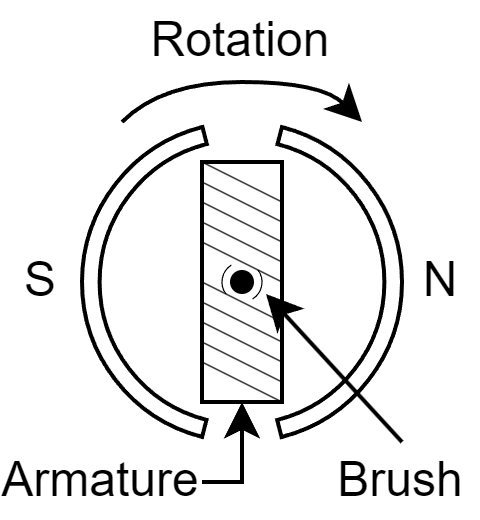
\includegraphics[width=0.25\linewidth]{images/brushed.png}
    \caption{Brushed motor structure}
\end{figure}

Continuously adjusting the current causes the armature to keep rotating and generating motion. 
This current modification is facilitated by two connectors positioned at the center of the armature, known as brushes. 
It's worth noting that in lower-cost electrical motors, the external magnets remain stationary. 
However, these budget-friendly versions encounter several issues related to their brushes:
\begin{itemize}
    \item Brushes gradually wear out over time.
    \item Brushes generate noise during operation.
    \item They impose a maximum speed limit.
    \item Cooling them proves to be challenging.
    \item They restrict the number of poles that can be utilized.
\end{itemize}
To circumvent this issue, one can opt for brushless motors, where external magnets are substituted with copper coils and a magnet is positioned at the center. 
This configuration yields a motor wherein brushes are replaced by electronics, permanent magnets reside on the rotor, and electromagnets are situated on the stator. 
While these motors offer superior performance, they also come at a higher cost compared to their brushed counterparts.

\begin{figure}[H]
    \centering
    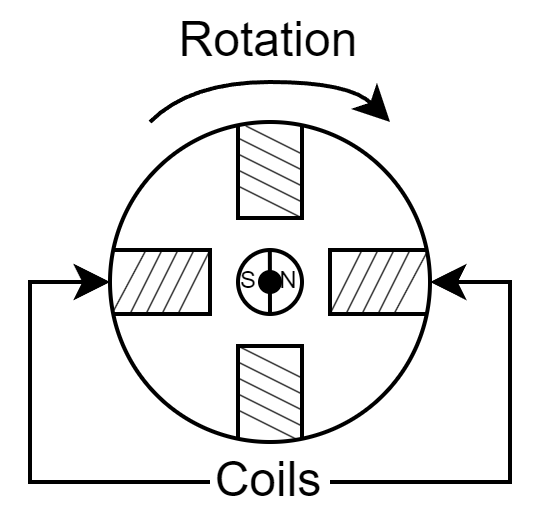
\includegraphics[width=0.25\linewidth]{images/brushless.png}
    \caption{Brushless motor structure}
\end{figure}

\subsection{Stepper motor}
The stepper motor, a type of synchronous electric motor lacking brushes, transforms digital pulses into mechanical shaft rotations.

A stepper motor offers several advantages: it provides a direct correlation between input pulse and rotation angle, maintains full torque even at standstill when windings are energized, enables precise positioning and repeatability, responds promptly to starting, stopping, and reversing commands, boasts high reliability due to the absence of contact brushes, facilitates open-loop control which simplifies and reduces costs, supports very low-speed synchronous rotation with directly coupled loads, and offers a wide range of rotational speeds.
However, there are also disadvantages: it necessitates a specialized control circuit, consumes more current compared to DC motors, experiences a reduction in torque at higher speeds, risks resonances if not adequately managed, and finds it challenging to operate at extremely high speeds.

\begin{figure}[H]
    \centering
    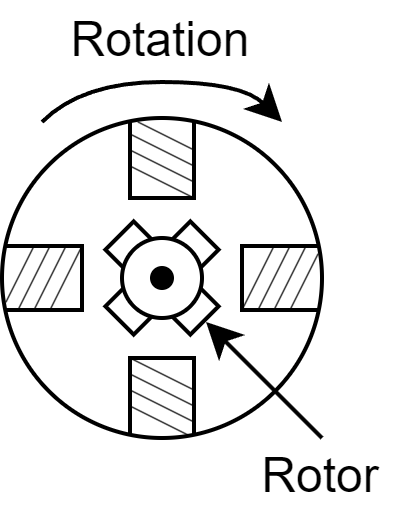
\includegraphics[width=0.2\linewidth]{images/stepper.png}
    \caption{Stepper motor structure}
\end{figure}

The step angle, denoted by $\varphi$, can be determined using the following formula:
\[\varphi =\left(\dfrac{N_s-N_r}{N_s \cdot N_r}\right) \times 360^\circ\]
In this equation, $N_s$ represents the number of teeth on the stator, and $N_r$ represents the number of teeth on the rotor.

\subsection{Servo motor}
A servo is a type of specialized motor designed to precisely move its shaft to a specific position. These motors find common use in hobby radio control applications. 
They possess the capability to measure their own position and adjust for external loads in accordance with a control signal.

Servo motors are typically constructed from direct current motors with additional components including gear reduction, a position sensor, and control electronics. 
The travel range of the shaft is usually limited to 180 degrees, which is adequate for the majority of applications.